% Options for packages loaded elsewhere
\PassOptionsToPackage{unicode}{hyperref}
\PassOptionsToPackage{hyphens}{url}
%
\documentclass[
]{book}
\usepackage{lmodern}
\usepackage{amssymb,amsmath}
\usepackage{ifxetex,ifluatex}
\ifnum 0\ifxetex 1\fi\ifluatex 1\fi=0 % if pdftex
  \usepackage[T1]{fontenc}
  \usepackage[utf8]{inputenc}
  \usepackage{textcomp} % provide euro and other symbols
\else % if luatex or xetex
  \usepackage{unicode-math}
  \defaultfontfeatures{Scale=MatchLowercase}
  \defaultfontfeatures[\rmfamily]{Ligatures=TeX,Scale=1}
\fi
% Use upquote if available, for straight quotes in verbatim environments
\IfFileExists{upquote.sty}{\usepackage{upquote}}{}
\IfFileExists{microtype.sty}{% use microtype if available
  \usepackage[]{microtype}
  \UseMicrotypeSet[protrusion]{basicmath} % disable protrusion for tt fonts
}{}
\makeatletter
\@ifundefined{KOMAClassName}{% if non-KOMA class
  \IfFileExists{parskip.sty}{%
    \usepackage{parskip}
  }{% else
    \setlength{\parindent}{0pt}
    \setlength{\parskip}{6pt plus 2pt minus 1pt}}
}{% if KOMA class
  \KOMAoptions{parskip=half}}
\makeatother
\usepackage{xcolor}
\IfFileExists{xurl.sty}{\usepackage{xurl}}{} % add URL line breaks if available
\IfFileExists{bookmark.sty}{\usepackage{bookmark}}{\usepackage{hyperref}}
\hypersetup{
  pdftitle={16s rRNA analysis workshop},
  pdfauthor={Hena R. Ramay},
  hidelinks,
  pdfcreator={LaTeX via pandoc}}
\urlstyle{same} % disable monospaced font for URLs
\usepackage{color}
\usepackage{fancyvrb}
\newcommand{\VerbBar}{|}
\newcommand{\VERB}{\Verb[commandchars=\\\{\}]}
\DefineVerbatimEnvironment{Highlighting}{Verbatim}{commandchars=\\\{\}}
% Add ',fontsize=\small' for more characters per line
\usepackage{framed}
\definecolor{shadecolor}{RGB}{248,248,248}
\newenvironment{Shaded}{\begin{snugshade}}{\end{snugshade}}
\newcommand{\AlertTok}[1]{\textcolor[rgb]{0.94,0.16,0.16}{#1}}
\newcommand{\AnnotationTok}[1]{\textcolor[rgb]{0.56,0.35,0.01}{\textbf{\textit{#1}}}}
\newcommand{\AttributeTok}[1]{\textcolor[rgb]{0.77,0.63,0.00}{#1}}
\newcommand{\BaseNTok}[1]{\textcolor[rgb]{0.00,0.00,0.81}{#1}}
\newcommand{\BuiltInTok}[1]{#1}
\newcommand{\CharTok}[1]{\textcolor[rgb]{0.31,0.60,0.02}{#1}}
\newcommand{\CommentTok}[1]{\textcolor[rgb]{0.56,0.35,0.01}{\textit{#1}}}
\newcommand{\CommentVarTok}[1]{\textcolor[rgb]{0.56,0.35,0.01}{\textbf{\textit{#1}}}}
\newcommand{\ConstantTok}[1]{\textcolor[rgb]{0.00,0.00,0.00}{#1}}
\newcommand{\ControlFlowTok}[1]{\textcolor[rgb]{0.13,0.29,0.53}{\textbf{#1}}}
\newcommand{\DataTypeTok}[1]{\textcolor[rgb]{0.13,0.29,0.53}{#1}}
\newcommand{\DecValTok}[1]{\textcolor[rgb]{0.00,0.00,0.81}{#1}}
\newcommand{\DocumentationTok}[1]{\textcolor[rgb]{0.56,0.35,0.01}{\textbf{\textit{#1}}}}
\newcommand{\ErrorTok}[1]{\textcolor[rgb]{0.64,0.00,0.00}{\textbf{#1}}}
\newcommand{\ExtensionTok}[1]{#1}
\newcommand{\FloatTok}[1]{\textcolor[rgb]{0.00,0.00,0.81}{#1}}
\newcommand{\FunctionTok}[1]{\textcolor[rgb]{0.00,0.00,0.00}{#1}}
\newcommand{\ImportTok}[1]{#1}
\newcommand{\InformationTok}[1]{\textcolor[rgb]{0.56,0.35,0.01}{\textbf{\textit{#1}}}}
\newcommand{\KeywordTok}[1]{\textcolor[rgb]{0.13,0.29,0.53}{\textbf{#1}}}
\newcommand{\NormalTok}[1]{#1}
\newcommand{\OperatorTok}[1]{\textcolor[rgb]{0.81,0.36,0.00}{\textbf{#1}}}
\newcommand{\OtherTok}[1]{\textcolor[rgb]{0.56,0.35,0.01}{#1}}
\newcommand{\PreprocessorTok}[1]{\textcolor[rgb]{0.56,0.35,0.01}{\textit{#1}}}
\newcommand{\RegionMarkerTok}[1]{#1}
\newcommand{\SpecialCharTok}[1]{\textcolor[rgb]{0.00,0.00,0.00}{#1}}
\newcommand{\SpecialStringTok}[1]{\textcolor[rgb]{0.31,0.60,0.02}{#1}}
\newcommand{\StringTok}[1]{\textcolor[rgb]{0.31,0.60,0.02}{#1}}
\newcommand{\VariableTok}[1]{\textcolor[rgb]{0.00,0.00,0.00}{#1}}
\newcommand{\VerbatimStringTok}[1]{\textcolor[rgb]{0.31,0.60,0.02}{#1}}
\newcommand{\WarningTok}[1]{\textcolor[rgb]{0.56,0.35,0.01}{\textbf{\textit{#1}}}}
\usepackage{longtable,booktabs}
% Correct order of tables after \paragraph or \subparagraph
\usepackage{etoolbox}
\makeatletter
\patchcmd\longtable{\par}{\if@noskipsec\mbox{}\fi\par}{}{}
\makeatother
% Allow footnotes in longtable head/foot
\IfFileExists{footnotehyper.sty}{\usepackage{footnotehyper}}{\usepackage{footnote}}
\makesavenoteenv{longtable}
\usepackage{graphicx,grffile}
\makeatletter
\def\maxwidth{\ifdim\Gin@nat@width>\linewidth\linewidth\else\Gin@nat@width\fi}
\def\maxheight{\ifdim\Gin@nat@height>\textheight\textheight\else\Gin@nat@height\fi}
\makeatother
% Scale images if necessary, so that they will not overflow the page
% margins by default, and it is still possible to overwrite the defaults
% using explicit options in \includegraphics[width, height, ...]{}
\setkeys{Gin}{width=\maxwidth,height=\maxheight,keepaspectratio}
% Set default figure placement to htbp
\makeatletter
\def\fps@figure{htbp}
\makeatother
\setlength{\emergencystretch}{3em} % prevent overfull lines
\providecommand{\tightlist}{%
  \setlength{\itemsep}{0pt}\setlength{\parskip}{0pt}}
\setcounter{secnumdepth}{5}
\usepackage{booktabs}
\usepackage[]{natbib}
\bibliographystyle{apalike}

\title{16s rRNA analysis workshop}
\author{Hena R. Ramay}
\date{2020-06-16}

\begin{document}
\maketitle

{
\setcounter{tocdepth}{1}
\tableofcontents
}
\hypertarget{introduction}{%
\chapter{Introduction}\label{introduction}}

Our intention is to develop workshop material as we go along. For each day of the workshop, the basic material will be uploaded and more details will be added based on your questions and problems we encounter. So please ask as many questions are you can to help us in making this workshop better!!

\hypertarget{workshop-schedule}{%
\section{Workshop Schedule}\label{workshop-schedule}}

We will try to cover the following material in the course:

\begin{itemize}
\tightlist
\item
  Day1

  \begin{itemize}
  \tightlist
  \item
    9:00 - 9:45 am Introductions and a presentation of the basic concepts
  \item
    9:45 - 10:30 am CutAdapt- how remove primers
  \item
    10:30 - 10:45 am Break
  \item
    10:45 - 12 pm Installations of the required packages and data download
  \item
    12 - 1 pm Lunch break
  \item
    1 - 3 pm Reading data in and inspecting read quality
  \end{itemize}
\item
  Day2

  \begin{itemize}
  \tightlist
  \item
    9:30 -10:30 am Filter and trim + learn error rates + Sample inference + Merge samples
  \item
    10:30 - 10:45 am Break
  \item
    10:45 - 12 Generate sequence table and remove Chimeras
  \item
    12 - 1 pm Lunch break
  \item
    1 - 2 pm Taxonomy explanation + assign your sequences. If time permits, make a phyloseq object
  \item
    2 - 4 pm on wards we will use a real world dataset to re-do what we have learned here
  \end{itemize}
\end{itemize}

\hypertarget{important-links}{%
\section{Important links}\label{important-links}}

\begin{itemize}
\tightlist
\item
  DADA2 Tutorial : \href{http://benjjneb.github.io/dada2/tutorial.html}{link}
\item
  Day One presentation : \href{microbiomeworkshop.pdf}{link}
\item
  Day One dataset : \href{MiSeqSOPData.zip}{link}
\item
  Project dataset : \href{https://www.dropbox.com/sh/qra6ohbsyt1icaz/AAACvlNjUhfkbkGIp_1KA2uCa?dl=0}{link}
\end{itemize}

\hypertarget{basic-information}{%
\chapter{Basic Information}\label{basic-information}}

We are very excited to teach this workshop and share what we know with you all !

So lets start by talking about the very basics:

\hypertarget{what-are-we-trying-to-achieve}{%
\section{What are we trying to achieve}\label{what-are-we-trying-to-achieve}}

Our goal is very similar to gathering data on a city neighbourhood to find out who lives there, how the demographic changes over time or in case of a drastic event. We can gather more information by asking about neighbours, quality of life etc. Similarly when we are looking at microbial communities our first question is who is there, how abundant and how their presence changes over time or when conditions change. We can also ask questions like how the microbiomes are interacting with each other (metabolites).

For the scope of this workshop we will stick to the simple questions: who and how much?

\hypertarget{basics-background}{%
\section{Basics \& Background}\label{basics-background}}

Here is the link to the lecture we will start with today: \href{microbiomeworkshop.pdf}{workshop}

Key points are:

\begin{itemize}
\tightlist
\item
  Think of a hypothesis before doing an experiment
\item
  Spend time on experiment design.

  \begin{itemize}
  \tightlist
  \item
    Sample size, 16s region to amplify etc
  \item
    Talk to a bioinformatician
  \item
    Think about the depth of sequencing if you want to capture the less abundant taxa
  \item
    Add negative control to account for contamination
  \end{itemize}
\item
  Thoughtful data analysis is critical for successful identification of microbes
\end{itemize}

``If you torture the data long enough, it will confess.''- Ronald Coase, Economist

\hypertarget{primer-removal}{%
\chapter{Primer Removal}\label{primer-removal}}

There are multiple ways in which you can remove primers sequences from your fastq files.
\href{https://cutadapt.readthedocs.io/en/stable/index.html}{CutAdapt} and \href{http://www.usadellab.org/cms/?page=trimmomatic}{trimmomatic} are two widely used tools for short-read data. DADA2 package has its own removePrimers sequence function which is recommended for PacBio data.

\hypertarget{cutadapt}{%
\section{CutAdapt}\label{cutadapt}}

The first step that everyone performs before doing an analysis is data cleaning. Data cleaning can mean multiple things in this context: primer removal, quality trimming, removing very short sequences etc. Remember inconsistent and incorrect data leads to false conclusions. In short, garbage in, garbage out applies to all data.

The first step that we will do with amplicon data is check which 16s rRNA gene region was sequenced, find the primer that were used and remove them. For this purpose there are a few software available like, cutAdapt, Trimmomatic, skewer. For the purpose of this workshop we will use cutAdapt.

Cutadapt finds and removes adapter sequences, primers, poly-A tails and other types of unwanted sequence from your high-throughput sequencing reads. It also alows you to perform quality trimming on your reads.

\hypertarget{primer-removal-for-paired-end-reads}{%
\subsection{Primer removal for paired end reads}\label{primer-removal-for-paired-end-reads}}

Here, the input reads are in reads.1.fastq and reads.2.fastq, and the result will be written to out.1.fastq and out.2.fastq.

In paired-end mode, the options -a, -b, -g and -u that also exist in single-end mode are applied to the forward reads only. To modify the reverse read, these options have uppercase versions -A, -B, -G and -U that work just like their counterparts. In the example above, ADAPTER\_FWD will therefore be trimmed from the forward reads and ADAPTER\_REV from the reverse reads.

\begin{longtable}[]{@{}ll@{}}
\toprule
Single-end/R1 option & Corresponding option for R2\tabularnewline
\midrule
\endhead
--adapter, -a & -A\tabularnewline
--front, -g & -G\tabularnewline
--anywhere, -b & -B\tabularnewline
--cut, -u & -U\tabularnewline
--output, -o & --paired-output, -p\tabularnewline
\bottomrule
\end{longtable}

In paired-end mode, Cutadapt checks whether the input files are properly paired. An error is raised if one of the files contains more reads than the other or if the read names in the two files do not match. The read name comparison ignores a trailing /1 or /2 to allow processing some old Illumina paired-end files.

Cutadapt supports compressed input and output files. Whether an input file needs to be decompressed or an output file needs to be compressed is detected automatically by inspecting the file name: For example, if it ends in .gz, then gzip compression is assumed

\hypertarget{quality-trimming}{%
\subsection{Quality trimming}\label{quality-trimming}}

-q 15,10

\hypertarget{call-cutadapt-from-r}{%
\subsection{Call cutAdapt from R}\label{call-cutadapt-from-r}}

Follow this link to see how you can call cutAdapt from within R
\url{https://benjjneb.github.io/dada2/ITS_workflow.html}

\hypertarget{dada2}{%
\chapter{DADA2}\label{dada2}}

\hypertarget{dada2-pipeline-v1.2}{%
\section{DADA2 pipeline (v1.2)}\label{dada2-pipeline-v1.2}}

From now on, we will be working on the DADA2 package version 1.12. DADA2 has great documentation and an excellent tutorial online.Please go to the following link \url{http://benjjneb.github.io/dada2/tutorial.html}

All the notes from now on are my additional comments to help you follow the pipeline:

\hypertarget{data-for-the-tutorial}{%
\subsection{Data for the tutorial}\label{data-for-the-tutorial}}

The data to use for the tutorial can be downloaded from \href{MiSeqSOPData.zip}{here}

\hypertarget{getting-ready-load-packages-and-get-file-list}{%
\subsection{Getting ready ( load packages and get file list)}\label{getting-ready-load-packages-and-get-file-list}}

Functions that we will be using here are :

\begin{itemize}
\tightlist
\item
  list.files()
\item
  sort()
\item
  strsplit()
\item
  basename()
\item
  sapply()
\end{itemize}

\hypertarget{inspect-read-quality-profiles}{%
\subsection{Inspect read quality profiles}\label{inspect-read-quality-profiles}}

Read in files

\begin{Shaded}
\begin{Highlighting}[]
\KeywordTok{library}\NormalTok{(dada2);}
\KeywordTok{library}\NormalTok{(limma)}
\NormalTok{path <-}\StringTok{ "MiSeq_SOP/"}
\KeywordTok{list.files}\NormalTok{(path)}
\end{Highlighting}
\end{Shaded}

\begin{verbatim}
##  [1] "F3D0_S188_L001_R1_001.fastq"   "F3D0_S188_L001_R2_001.fastq"  
##  [3] "F3D1_S189_L001_R1_001.fastq"   "F3D1_S189_L001_R2_001.fastq"  
##  [5] "F3D141_S207_L001_R1_001.fastq" "F3D141_S207_L001_R2_001.fastq"
##  [7] "F3D142_S208_L001_R1_001.fastq" "F3D142_S208_L001_R2_001.fastq"
##  [9] "F3D143_S209_L001_R1_001.fastq" "F3D143_S209_L001_R2_001.fastq"
## [11] "F3D144_S210_L001_R1_001.fastq" "F3D144_S210_L001_R2_001.fastq"
## [13] "F3D145_S211_L001_R1_001.fastq" "F3D145_S211_L001_R2_001.fastq"
## [15] "F3D146_S212_L001_R1_001.fastq" "F3D146_S212_L001_R2_001.fastq"
## [17] "F3D147_S213_L001_R1_001.fastq" "F3D147_S213_L001_R2_001.fastq"
## [19] "F3D148_S214_L001_R1_001.fastq" "F3D148_S214_L001_R2_001.fastq"
## [21] "F3D149_S215_L001_R1_001.fastq" "F3D149_S215_L001_R2_001.fastq"
## [23] "F3D150_S216_L001_R1_001.fastq" "F3D150_S216_L001_R2_001.fastq"
## [25] "F3D2_S190_L001_R1_001.fastq"   "F3D2_S190_L001_R2_001.fastq"  
## [27] "F3D3_S191_L001_R1_001.fastq"   "F3D3_S191_L001_R2_001.fastq"  
## [29] "F3D5_S193_L001_R1_001.fastq"   "F3D5_S193_L001_R2_001.fastq"  
## [31] "F3D6_S194_L001_R1_001.fastq"   "F3D6_S194_L001_R2_001.fastq"  
## [33] "F3D7_S195_L001_R1_001.fastq"   "F3D7_S195_L001_R2_001.fastq"  
## [35] "F3D8_S196_L001_R1_001.fastq"   "F3D8_S196_L001_R2_001.fastq"  
## [37] "F3D9_S197_L001_R1_001.fastq"   "F3D9_S197_L001_R2_001.fastq"  
## [39] "filtered"                      "HMP_MOCK.v35.fasta"           
## [41] "Mock_S280_L001_R1_001.fastq"   "Mock_S280_L001_R2_001.fastq"  
## [43] "mouse.dpw.metadata"            "mouse.time.design"            
## [45] "stability.batch"               "stability.files"
\end{verbatim}

\begin{Shaded}
\begin{Highlighting}[]
\CommentTok{# Forward and reverse fastq filenames have format: SAMPLENAME_R1_001.fastq and SAMPLENAME_R2_001.fastq}
\NormalTok{fnFs <-}\StringTok{ }\KeywordTok{sort}\NormalTok{(}\KeywordTok{list.files}\NormalTok{(path, }\DataTypeTok{pattern=}\StringTok{"_R1_001.fastq"}\NormalTok{, }\DataTypeTok{full.names =} \OtherTok{TRUE}\NormalTok{))}
\NormalTok{fnRs <-}\StringTok{ }\KeywordTok{sort}\NormalTok{(}\KeywordTok{list.files}\NormalTok{(path, }\DataTypeTok{pattern=}\StringTok{"_R2_001.fastq"}\NormalTok{, }\DataTypeTok{full.names =} \OtherTok{TRUE}\NormalTok{))}
\CommentTok{# Extract sample names, assuming filenames have format: SAMPLENAME_XXX.fastq}


\NormalTok{tmp<-}\KeywordTok{strsplit}\NormalTok{(}\KeywordTok{basename}\NormalTok{(fnFs), }\StringTok{"_"}\NormalTok{)}


\CommentTok{# As tmp is a list of vectors, we will have to use sapply function to get the first position out from each vector. The symbol '[' tells sapplly function that it is a vector and 1 specifies the vector index}

\NormalTok{samples.names<-}\KeywordTok{sapply}\NormalTok{(tmp,}\StringTok{'['}\NormalTok{,}\DecValTok{1}\NormalTok{)}
\end{Highlighting}
\end{Shaded}

\hypertarget{lets-make-plots-to-look-at-the-quality-for-multiple-files}{%
\subsection{Lets make plots to look at the quality for multiple files}\label{lets-make-plots-to-look-at-the-quality-for-multiple-files}}

\begin{Shaded}
\begin{Highlighting}[]
\KeywordTok{plotQualityProfile}\NormalTok{(fnFs[}\DecValTok{1}\OperatorTok{:}\DecValTok{2}\NormalTok{])}
\end{Highlighting}
\end{Shaded}

\begin{verbatim}
## Scale for 'y' is already present. Adding another scale for 'y', which will
## replace the existing scale.
\end{verbatim}

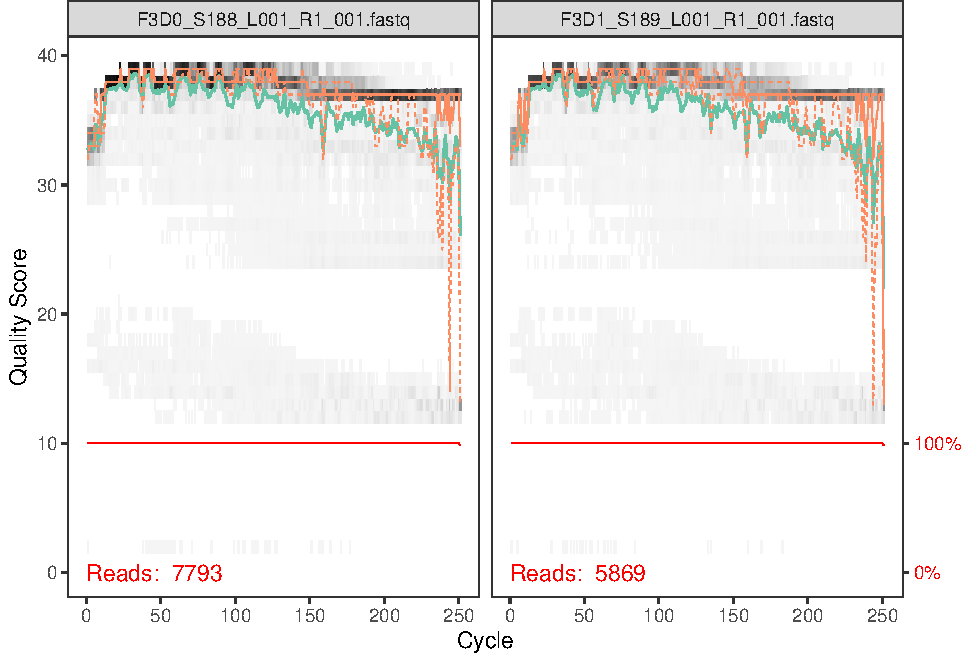
\includegraphics{16sworkshop_files/figure-latex/make_plots-1.pdf}

\begin{Shaded}
\begin{Highlighting}[]
\NormalTok{joint_fnames<-}\KeywordTok{c}\NormalTok{(}\KeywordTok{rbind}\NormalTok{(fnFs,fnRs))}

\KeywordTok{plotQualityProfile}\NormalTok{(joint_fnames)}
\end{Highlighting}
\end{Shaded}

\begin{verbatim}
## Scale for 'y' is already present. Adding another scale for 'y', which will
## replace the existing scale.
\end{verbatim}

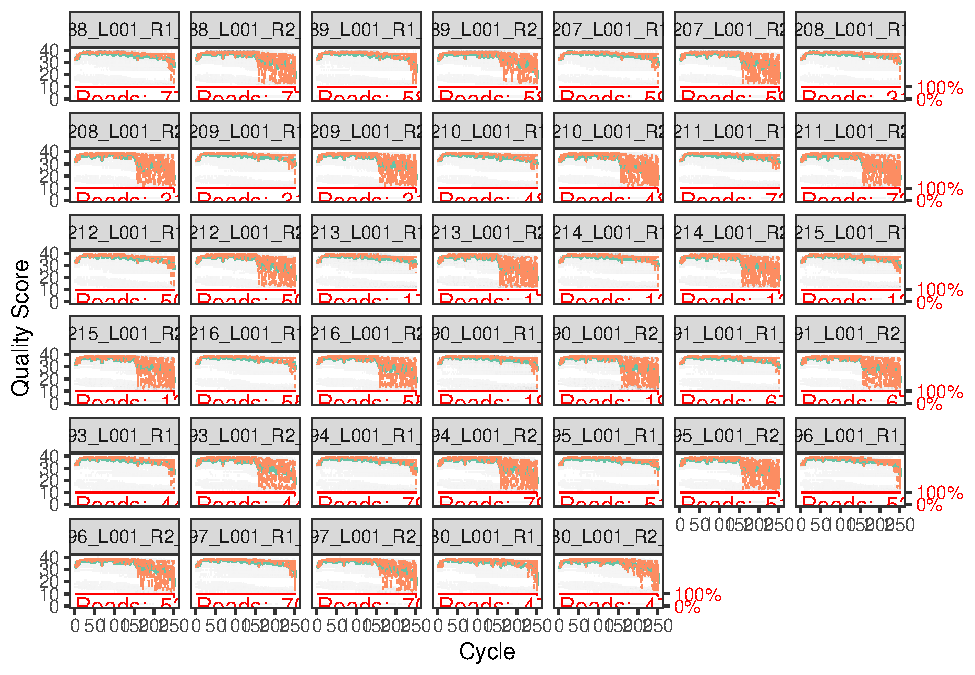
\includegraphics{16sworkshop_files/figure-latex/make_plots-2.pdf}

if there are too many files, use arrangegrob. See here \href{https://cran.r-project.org/web/packages/gridExtra/vignettes/arrangeGrob.html}{here} for details

For the rest of the DADA2 pipelien please \href{https://benjjneb.github.io/dada2/tutorial.html}{visit}

\hypertarget{some-tips}{%
\section{Some tips:}\label{some-tips}}

\begin{enumerate}
\def\labelenumi{\arabic{enumi}.}
\item
  At every step check how many reads are getting filtered. This is very important to make sure that you are not losing too much data.
\item
  If in the filtering step you are losing too many reads, relax the maxEE from 2 to 3 or more. Also check the length that you are truncating at.
\item
  If you are using cutAdapt for quality trimming, you don't have to use truncation in filterandtrim function of DADA2
\item
  Always keep in mind the overlap length for your region of interest. see the figure below for calculation:
\end{enumerate}

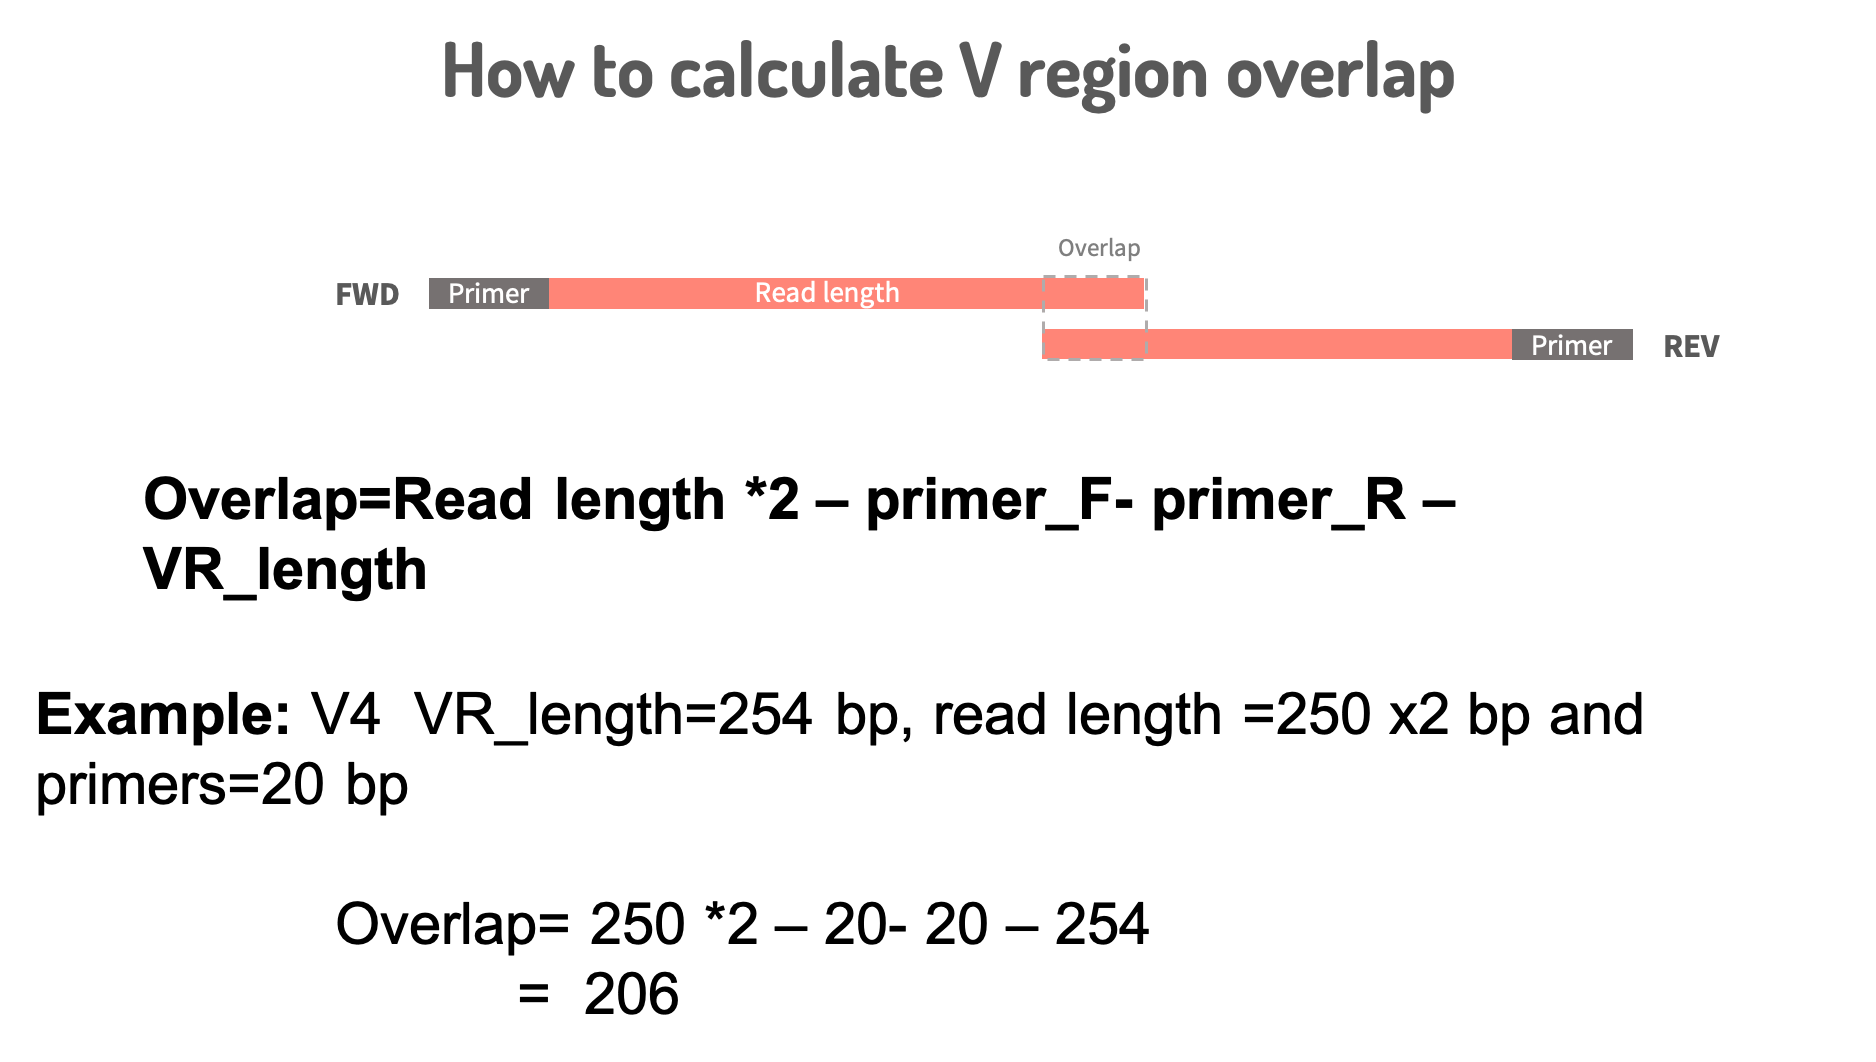
\includegraphics{overlap.png}

\begin{enumerate}
\def\labelenumi{\arabic{enumi}.}
\setcounter{enumi}{4}
\tightlist
\item
  If you lose too many sequences to chimera removal, please check that the primers are removed properly.
\end{enumerate}

\hypertarget{day-two}{%
\chapter{Day Two}\label{day-two}}

\hypertarget{main-concepts-to-be-discussed}{%
\section{Main concepts to be discussed:}\label{main-concepts-to-be-discussed}}

\begin{itemize}
\tightlist
\item
  Finish dada2 pipeline
\item
  Assign Taxonomy
\item
  Intro to Phyolseq package
\item
  Create a Phylum level bar plots
\item
  Alpha diversity plots
\item
  Beta diversity plots
\end{itemize}

Once we are finished using the dada2 package, we will have a sequence table and taxonomy table.

Lets look at the metadata files we have to get more information about these samples.

\begin{Shaded}
\begin{Highlighting}[]
\KeywordTok{library}\NormalTok{(ggplot2)}
\KeywordTok{library}\NormalTok{(dplyr)}
\NormalTok{time_info<-}\KeywordTok{read.delim}\NormalTok{(}\StringTok{"~/projects/16sanalysis_workshop/workshoptutorial/MiSeq_SOP/mouse.time.design"}\NormalTok{,}\DataTypeTok{sep  =} \StringTok{"}\CharTok{\textbackslash{}t}\StringTok{"}\NormalTok{)}
\NormalTok{dpw_info<-}\KeywordTok{read.delim}\NormalTok{(}\StringTok{"~/projects/16sanalysis_workshop/workshoptutorial/MiSeq_SOP/mouse.dpw.metadata"}\NormalTok{,}\DataTypeTok{sep  =} \StringTok{"}\CharTok{\textbackslash{}t}\StringTok{"}\NormalTok{)}

\NormalTok{sample_info<-}\KeywordTok{left_join}\NormalTok{(time_info,dpw_info,}\DataTypeTok{by=}\StringTok{"group"}\NormalTok{)}

\KeywordTok{rownames}\NormalTok{(sample_info)<-}\StringTok{ }\NormalTok{sample_info}\OperatorTok{$}\NormalTok{group}

\NormalTok{sample_info}
\end{Highlighting}
\end{Shaded}

\begin{verbatim}
##         group  time dpw
## F3D0     F3D0 Early   0
## F3D1     F3D1 Early   1
## F3D141 F3D141  Late 141
## F3D142 F3D142  Late 142
## F3D143 F3D143  Late 143
## F3D144 F3D144  Late 144
## F3D145 F3D145  Late 145
## F3D146 F3D146  Late 146
## F3D147 F3D147  Late 147
## F3D148 F3D148  Late 148
## F3D149 F3D149  Late 149
## F3D150 F3D150  Late 150
## F3D2     F3D2 Early   2
## F3D3     F3D3 Early   3
## F3D5     F3D5 Early   5
## F3D6     F3D6 Early   6
## F3D7     F3D7 Early   7
## F3D8     F3D8 Early   8
## F3D9     F3D9 Early   9
\end{verbatim}

Lets make a phyloseq object

Now that we have sample\_info lets try to make a phyloseq object out of this

\begin{Shaded}
\begin{Highlighting}[]
\KeywordTok{library}\NormalTok{(phyloseq)}
\NormalTok{taxa<-}\KeywordTok{readRDS}\NormalTok{(}\StringTok{"~/projects/16sanalysis_workshop/workshoptutorial/output/taxa.rds"}\NormalTok{)}
\NormalTok{seq<-}\KeywordTok{readRDS}\NormalTok{(}\StringTok{"~/projects/16sanalysis_workshop/workshoptutorial/output/seq.rds"}\NormalTok{)}

\NormalTok{ps <-}\StringTok{ }\KeywordTok{phyloseq}\NormalTok{(}\KeywordTok{otu_table}\NormalTok{(seq,}\DataTypeTok{taxa_are_rows =}\NormalTok{ F),}
               \KeywordTok{sample_data}\NormalTok{(sample_info),}
               \KeywordTok{tax_table}\NormalTok{(taxa))}

\NormalTok{ps}
\end{Highlighting}
\end{Shaded}

\begin{verbatim}
## phyloseq-class experiment-level object
## otu_table()   OTU Table:         [ 234 taxa and 19 samples ]
## sample_data() Sample Data:       [ 19 samples by 3 sample variables ]
## tax_table()   Taxonomy Table:    [ 234 taxa by 7 taxonomic ranks ]
\end{verbatim}

You can see that this object has an OTU table(ASV table), sample data and tax\_table. You can use functions tax\_table(), sample\_data() and otu\_table() to access the data.

Take a look at:

\begin{itemize}
\tightlist
\item
  subset\_samples()
\item
  subset\_taxa()
\item
  tax\_glom()
\item
  sample\_sums()
\item
  prune\_samples()
\item
  transform\_sample\_counts()
\item
  psmelt()
\end{itemize}

\begin{Shaded}
\begin{Highlighting}[]
\NormalTok{ps2<-}\KeywordTok{tax_glom}\NormalTok{(ps,}\DataTypeTok{taxrank =} \StringTok{"Phylum"}\NormalTok{)}
\NormalTok{ps2 =}\StringTok{ }\KeywordTok{transform_sample_counts}\NormalTok{(ps2, }\ControlFlowTok{function}\NormalTok{(x) x}\OperatorTok{/}\KeywordTok{sum}\NormalTok{(x))}
\NormalTok{pmelt<-}\KeywordTok{psmelt}\NormalTok{(ps2) }\OperatorTok\StringTok{ }\KeywordTok{arrange}\NormalTok{(}\KeywordTok{desc}\NormalTok{(Abundance))}

\NormalTok{cutoff<-}\FloatTok{0.005}
\NormalTok{pmelt_filt<-pmelt }\OperatorTok\StringTok{ }\KeywordTok{group_by}\NormalTok{(Phylum,time) }\OperatorTok\StringTok{ }\KeywordTok{filter}\NormalTok{(}\KeywordTok{sum}\NormalTok{(Abundance) }\OperatorTok{>}\NormalTok{cutoff)}

\KeywordTok{ggplot}\NormalTok{(pmelt_filt,}\KeywordTok{aes}\NormalTok{(}\DataTypeTok{x=}\NormalTok{Sample,}\DataTypeTok{y=}\NormalTok{Abundance,}\DataTypeTok{color=}\NormalTok{Phylum,}\DataTypeTok{fill=}\NormalTok{Phylum)) }\OperatorTok{+}\KeywordTok{geom_bar}\NormalTok{(}\DataTypeTok{stat =} \StringTok{"identity"}\NormalTok{)}
\end{Highlighting}
\end{Shaded}

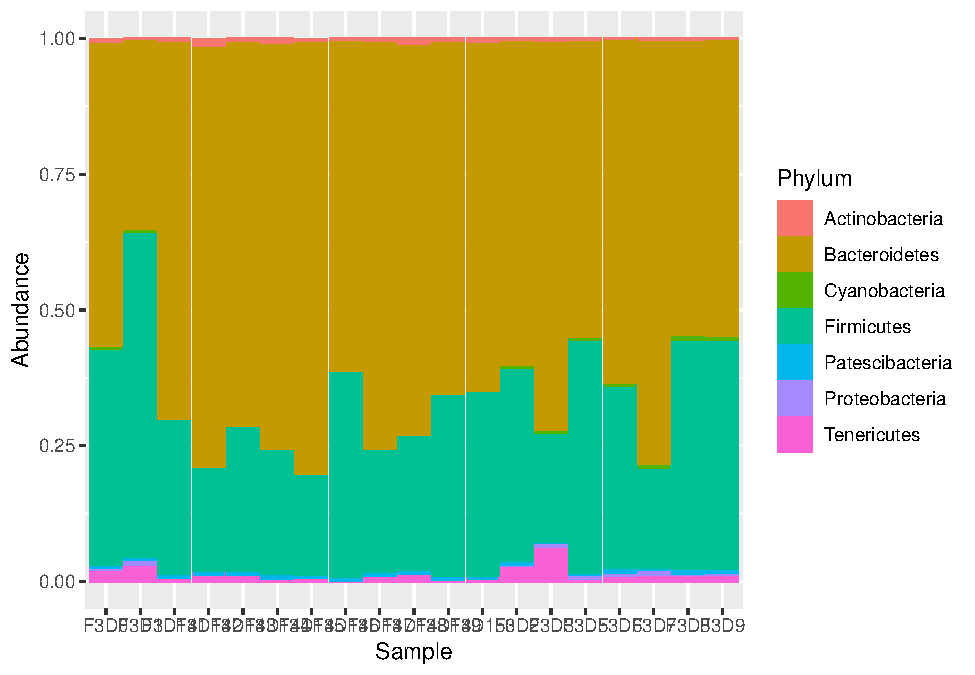
\includegraphics{16sworkshop_files/figure-latex/unnamed-chunk-2-1.pdf}

\begin{Shaded}
\begin{Highlighting}[]
\NormalTok{pmelt_filt }\OperatorTok\StringTok{ }\KeywordTok{group_by}\NormalTok{(time,Phylum) }\OperatorTok\StringTok{ }\KeywordTok{summarise}\NormalTok{(}\DataTypeTok{mean_Abundance=}\KeywordTok{mean}\NormalTok{(Abundance)) }\OperatorTok\StringTok{ }\KeywordTok{ggplot}\NormalTok{(.,}\KeywordTok{aes}\NormalTok{(}\DataTypeTok{x=}\NormalTok{time,}\DataTypeTok{y=}\NormalTok{mean_Abundance,}\DataTypeTok{fill=}\NormalTok{Phylum)) }\OperatorTok{+}\KeywordTok{geom_bar}\NormalTok{(}\DataTypeTok{stat=}\StringTok{"identity"}\NormalTok{)}
\end{Highlighting}
\end{Shaded}

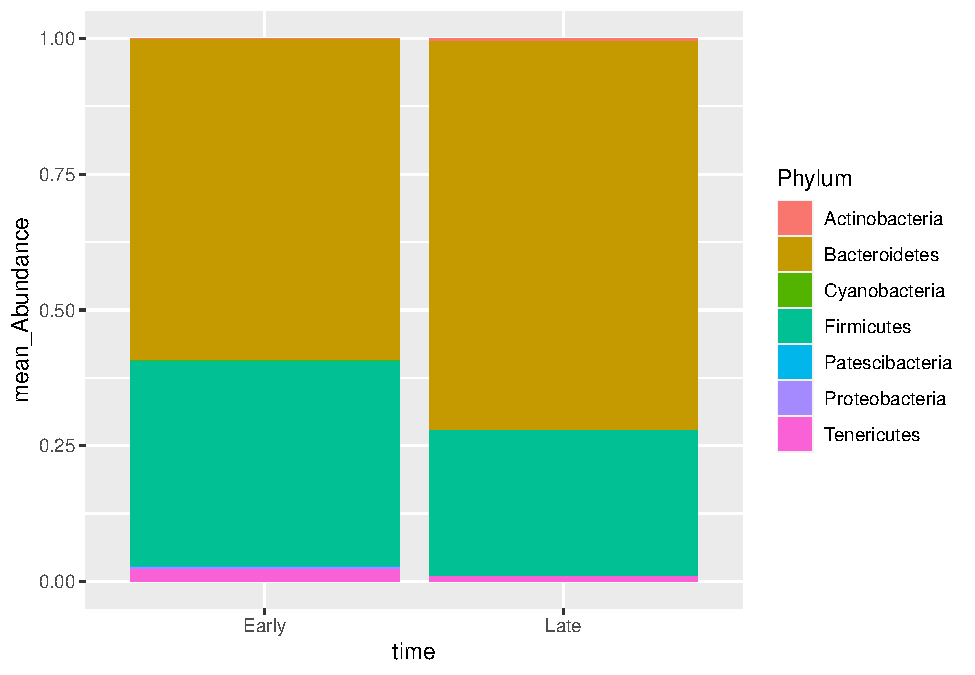
\includegraphics{16sworkshop_files/figure-latex/unnamed-chunk-2-2.pdf}

Figure out how to change the colors to custom colors!!

\begin{Shaded}
\begin{Highlighting}[]
\NormalTok{pmelt_filt }\OperatorTok\StringTok{ }\KeywordTok{group_by}\NormalTok{(time,Phylum) }\OperatorTok\StringTok{ }\KeywordTok{summarise}\NormalTok{(}\DataTypeTok{mean=}\KeywordTok{mean}\NormalTok{(Abundance))}
\end{Highlighting}
\end{Shaded}

\begin{verbatim}
## # A tibble: 12 x 3
## # Groups:   time [2]
##    time  Phylum              mean
##    <fct> <fct>              <dbl>
##  1 Early Actinobacteria  0.00133 
##  2 Early Bacteroidetes   0.592   
##  3 Early Cyanobacteria   0.000594
##  4 Early Firmicutes      0.378   
##  5 Early Patescibacteria 0.00285 
##  6 Early Proteobacteria  0.00331 
##  7 Early Tenericutes     0.0218  
##  8 Late  Actinobacteria  0.00472 
##  9 Late  Bacteroidetes   0.716   
## 10 Late  Firmicutes      0.269   
## 11 Late  Patescibacteria 0.000993
## 12 Late  Tenericutes     0.00845
\end{verbatim}

\hypertarget{alpha-beta-diversity}{%
\section{Alpha \& beta Diversity}\label{alpha-beta-diversity}}

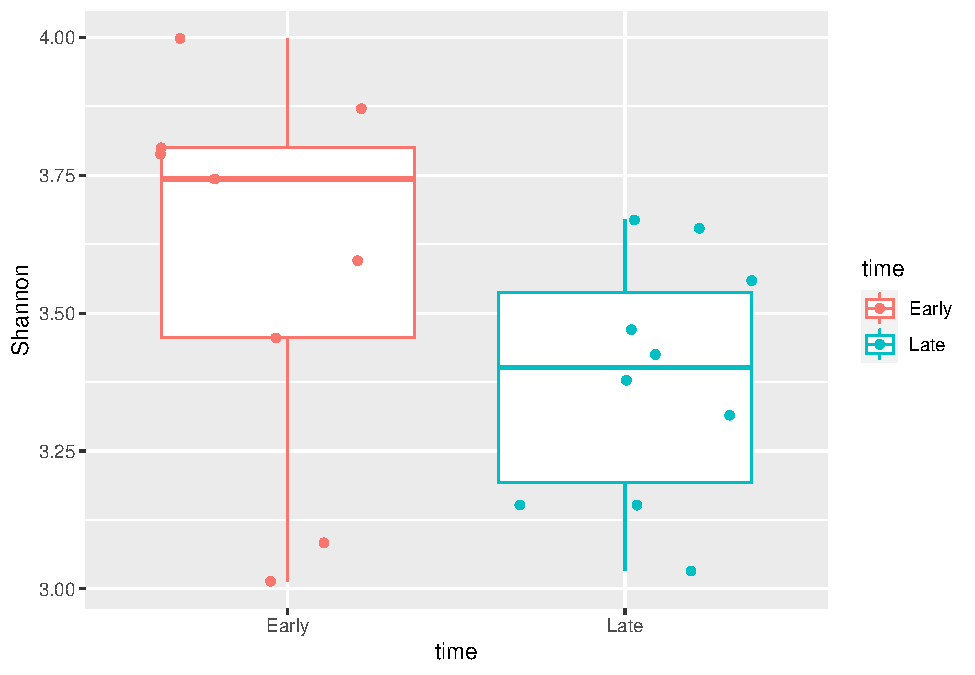
\includegraphics{16sworkshop_files/figure-latex/alpha diversit-1.pdf}

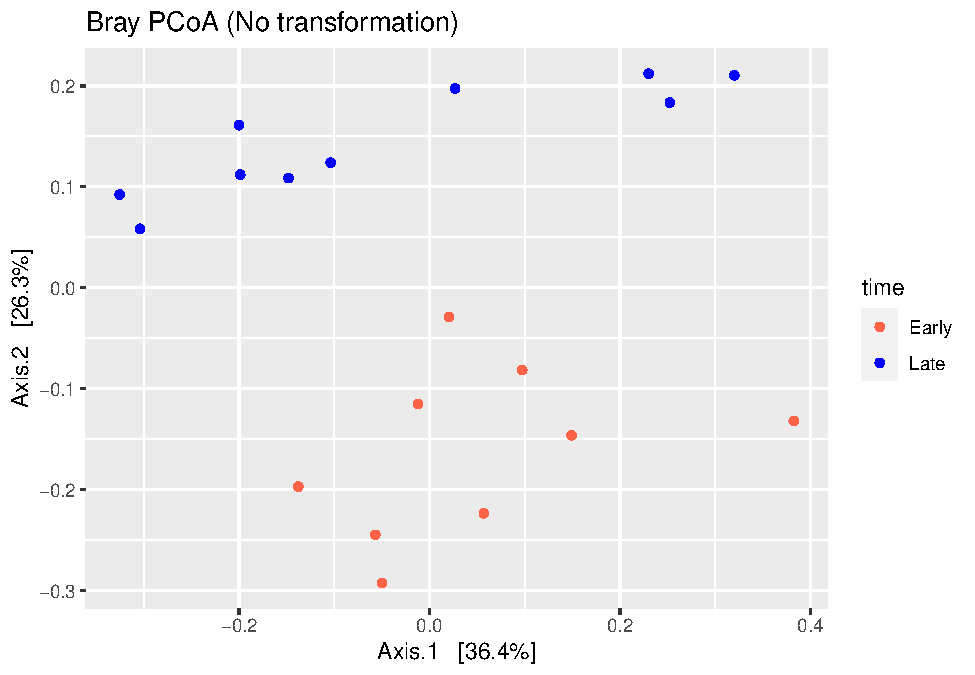
\includegraphics{16sworkshop_files/figure-latex/unnamed-chunk-3-1.pdf} 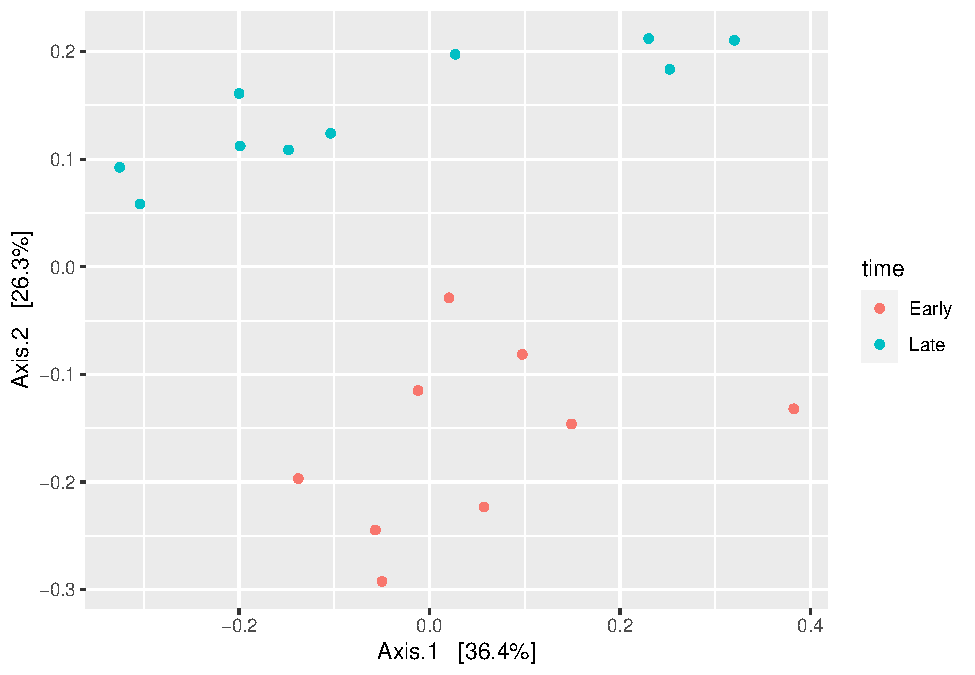
\includegraphics{16sworkshop_files/figure-latex/unnamed-chunk-3-2.pdf}

\hypertarget{summary}{%
\chapter{Summary}\label{summary}}

\hypertarget{what-next}{%
\chapter{What Next?}\label{what-next}}

What you have learnt so far is just the beginging!! There is a lot more ot learn and do.

For example, after looking at beta diversity, you can also look at differential abundance to see which taxa are different in each treatment group or over time.

Most commonly used methods for doing this is \href{https://bioconductor.org/packages/release/bioc/html/DESeq2.html}{deseq2} and a new one is \href{https://github.com/bryandmartin/corncob/}{corncob}. Before using them, please read the papers carefully to know the limitations and correct usage of these pacakages.

Some people also try to do functional analaysis with 16s data and for this \href{https://github.com/picrust/picrust2/wiki}{PICRUST2} pacakge is usually used.

  \bibliography{book.bib,packages.bib}

\end{document}
